%\chapter{SIZER: dataset e modello per l’analisi e l'apprendimento dell’abbigliamento 3D size sensitive}
\section{SIZER: dataset e modello per l’analisi e l'apprendimento dell’abbigliamento 3D size sensitive}

Esistono numerosi modelli nell’ambito dell’abbigliamento 3Dimensionale, progettati ed ottimizzati grazie a database costruiti su basi di dati reali.  
Nessuno di questi, però, è in grado di implementare la funzione di “deformare” l’abito in base alla taglia.

\medskip

\begin{itemize}
\item SizerNet in grado di prevedere le deformazioni 3D elaborate in tempo reale degli abiti condizionate in base ai parametri del corpo umano ed alle dimensioni dell’indumento 
\item ParserNet con l’obiettivo di decifrare e dedurre la struttura dei vestiti (e la loro forma), distinguendoli dal corpo umano tramite un singolo passaggio data una mesh in input.

\end{itemize}

\medskip

SizerNet apre la possibilità di stimare e visualizzare nel dettaglio la vestibilità di un indumento nelle sue varie taglie mentre ParserNet permette di modificare vestiti relativi alla mesh di input in maniera diretta e precisa, eliminando la necessità di scannerizzare le singole segmentazioni, problema molto impegnativo già in sé.

\medskip

In “SIZER: A Dataset and Model for Parsing 3D Clothing and Learning Size Sensitive 3D Clothing” (\url{https://virtualhumans.mpi-inf.mpg.de/papers/tiwari20sizer/sizer.pdf}) ci si focalizza sulla vestibilità di vestiti virtuali su scansioni 3D del corpo. Gli indumenti interagiscono con il corpo in modo complesso, e la vestibilità è una funzione non lineare di taglia e shape del corpo, per cui simulare tale vestibilità non è banale. Viene introdotto il dataset SIZER (\url{http://virtualhumans.mpi-inf.mpg.de/sizer/}), un dataset di circa 2000 scansioni 3D di 100 persone che indossano 10 tipi di vestiario in taglie diverse (S, M, L, XL), registrazioni sul modello SMPL, scansioni segmentate in tipi di vestiario, categorie di vestiti e taglie.
Con SIZER viene addestrata una rete neurale, SizerNet, che permette di stimare e visualizzare la vestibilità dei vestiti in base alla taglia, la human body shape e l’indumento dati in input. L’addestramento di SizerNet necessita di un mapping tra le scansioni e mesh multi-strato - mesh separate per il corpo e per i capi di sopra e di sotto. Per fare ciò, c’è bisogno di segmentare le scansioni 3D, stimare la body shape senza vestiti.
Dalle mesh multi-livello viene addestrato un codificatore in grado di mappare la mesh data in input ad un codice, ed un decodificatore che prende i parametri della forma del corpo di SMPL, la taglia dei vestiti dati in input e la taglia desiderata, per predire la vestibilità dei vestiti della taglia desiderata. A questo punto entra in gioco ParserNet, che mappa automaticamente la registrazione di una singola mesh ad una mesh multi-layer con un solo passo feed-forward. ParserNet non solo segmenta la singola mesh registration, ma riparametrizza la superficie in modo da renderla coerente con i template dei vestiti più comuni.
La rappresentazione multi-layer di ParserNet permette dunque di modificare i vestiti direttamente da una mesh data in input, eliminando la necessità di una segmentazione delle scansioni.
Vengono quindi utilizzate: una rete neurale che predice i parametri relativi alla posa, una per predire i parametri della forma, ParserNet, che fa la segmentazione (riconosce il corpo e i singoli vestiti) e SizerNet, che modifica la taglia dei vestiti: prende in input una mesh 3D e restituisce in output corpi 3D svestiti ad alta qualità, mantenendo l’identità del soggetto.
Il codice, il modello e il set di dati sono stati rilasciati all’indirizzo \url{https://virtualhumans.mpi-inf.mpg.de/sizer/}.

\newpage

\section{Dataset}

Il dataset SIZER, specifico nella variazione di taglia degli indumenti, comprende 2000 scansioni di 100 soggetti con diversa forma fisica, che indossano ciascuno due o tre taglie (S, M, L o XL) di differenti stili di abbigliamento casual. Vi sono 10 classi di indumenti, vale a dire shirt, dress-shirt (che si differenziano per la lunghezza della camicia), jeans, hoodie, polo t-shirt, t-shirt, shorts, vest, skirt e coat, ognuna contenente circa 200 scansioni.

\url{https://github.com/garvita-tiwari/sizer_dataset}

\medskip\medskip\medskip


\begin{figure}[ht!]
  \centering
  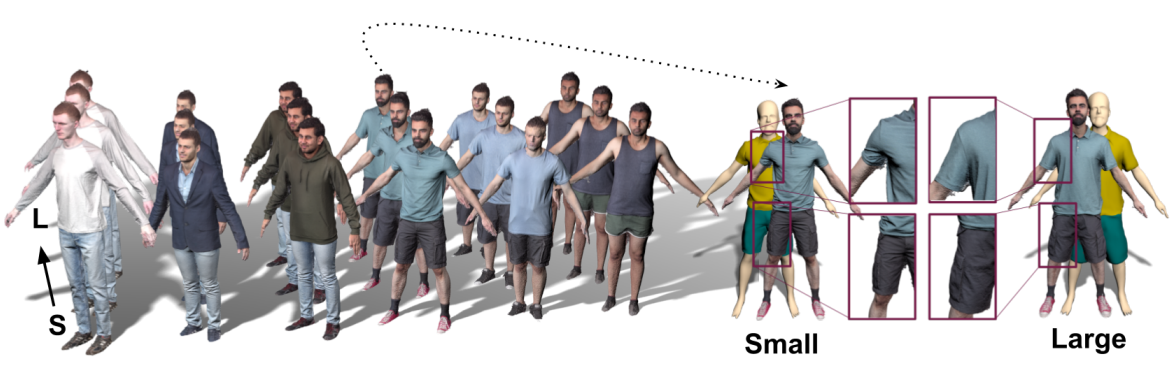
\includegraphics[scale=0.4]{Images/SizerPic/SizerDataset.png}
  \caption{(A sinistra): scansioni 3D di
persone in diversi stili e taglie di abbigliamento. (Destra): maglietta e pantaloncini
pantaloni per taglie piccole e grandi, che sono registrati su modelli comuni.}
  \label{fig:SizerDataset}
\end{figure}

\medskip\medskip\medskip

E’ stato scelto di catturare le mesh dei soggetti in una A-pose in modo tale da avere una vestibilità il più naturale e senza pieghe possibile.
Poiché le scansioni sono state acquisite mediante più di 130 fotocamere e ricostruite con il software \textit{Agisoft’s Metashape}, hanno alta risoluzione e i grafi delle diverse mesh che le rappresentano hanno differenti connessioni, quindi sarebbe difficoltoso utilizzare tale dataset, per questo motivo è stato necessario aggiungere al modello una fase di preprocessing del dataset, registrando le scansioni al modello SMPL.

\medskip\medskip\medskip

SMPL rappresenta il corpo umano come una funzione parametrica di posa e forma.
SMPL+G è una formulazione parametrica che permette di rappresentare corpo e vestiti come mesh separate. Per registrare gli indumenti bisogna per prima cosa segmentare le scansioni in modo da dividere le parti relative al corpo e quelle relative ai vestiti. Per ogni classe di vestiti si ottiene una mesh template definita come un subset del template di SMPL, dove ogni vertice dell’indumento è associato ad un vertice della forma fisica, come offset di quest’ultima.

\medskip

Dunque, il dataset contiene scansioni, scansioni segmentate, registrazioni SMPL+G, classi di indumenti e le taglie come etichette, ed è stato costruito per costruire un modello per l’estrazione di vestiti da una singola mesh (ParserNet) ed un resizing dei vestiti stessi (SizerNet).

\newpage

\begin{figure}[ht!]
  \centering
  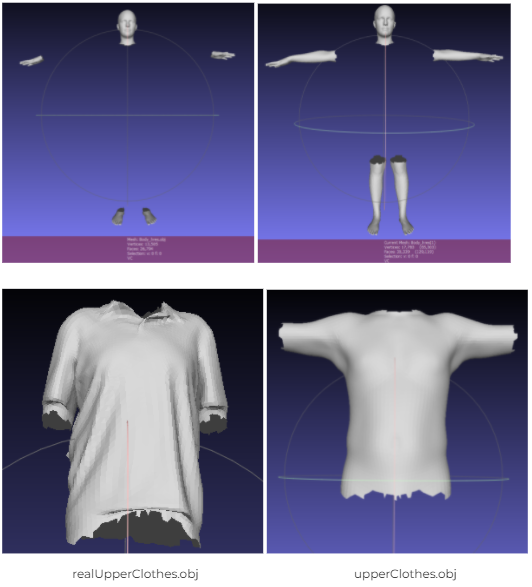
\includegraphics[scale=0.9]{Images/SizerPic/Sizer1.5.png}
    \label{fig:Sizer1.5}
\end{figure}

\medskip

Per ottenere il dataset è necessario andare alla sezione Data del sito \url{http://virtualhumans.mpi-inf.mpg.de/sizer/}.

\medskip

I soggetti delle scansioni di cui è composto il dataset hanno una età compresa tra i 19 e i 37 anni, con due sole eccezioni (51 e 69 anni). Per quel che riguarda l’altezza e il peso dei soggetti scansionati, invece, vi è un range piuttosto vasto, che permette una forte differenziazione dei dati.

\medskip

Il dataset è composto da scansioni di sole A-pose. Tali scansioni sono suddivise per genere e per tipologia di indumento (che può essere a maniche lunghe, maniche corte, pantalone lungo e pantalone corto). Come si può vedere dalle immagini seguenti, sono presenti anche gli oggetti utili a capire quali sezioni del corpo umano escludere dall’estrazione della superficie relativa agli abiti.

\newpage

Poiché il dataset SIZER include registrazioni sul modello SMPL , bisogna scaricare il modello SMPL \url{https://smpl.is.tue.mpg.de/}, che prende in input i parametri di forma e posa e restituisce il volume.

\medskip

\begin{figure}[ht!]
  \centering
  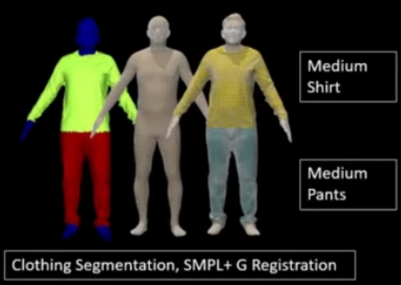
\includegraphics[scale=1]{Images/SizerPic/Sizer2.png}
    \label{fig:Sizer2}
\end{figure}

\paragraph{Preprocessing}
Il dataset SIZER è stato ottenuto tramite una feature extraction effettuata mediante due metodi illustrati di seguito nel dettaglio.

\subsection{Confronto tra SIZER e altri datasets}

Ad oggi, pochi dataset contengono scansioni di modelli tridimensionali relativi a soggetti e vestiti segmentati. Tra questi 3DPeople, Cloth3D consistono di un vasto dataset di rappresentazioni sintetiche di soggetti 3D vestiti. Ma non contengono deformazioni realistiche degli indumenti, come fa invece SIZER. THUman contiene sequenze di persone 3D con relativi abiti in movimento, catturati grazie ad un sensore RGBD (Kinectv2), e ricostruiti utilizzando un fusore volumetrico SDF. Tali scansioni, però, perdono di dettaglio rispetto alle scansioni 3D di SIZER e non vengono fornite le segmentazioni degli indumenti reali. Dyna e D-FAUST, invece, riguardano scansioni 3D ad alta risoluzione di  10 soggetti in movimento con forme differenti; l'unica pecca è che indossano solo vestiti "semplici". BUFF contiene scansioni ad alta risoluzione 3D di 6 soggetti con e senza abiti; neanche questo dataset tuttavia garantisce la segmentazione degli abiti: infatti è stato ideato per addestrare modelli per stimare solo la body shape che si trova al di sotto dei vestiti. 
DeepFashion3D riguarda scansioni di vari tipi di vestiti e potrebbe essere sostituito a SIZER per l'addestramento della rete neurale.








\newpage



\section{Metodo}




\medskip

Siccome queste scansioni sono ad alta risoluzione e rappresentate da mesh con diverse connettività ai grafi sottolineanti (ovvero grafi dove ogni arco direzionato viene sostituito con un vertice privo di direzione) risulta complicato utilizzare tale dataset per qualsiasi modello di apprendimento. Per questo motivo è necessario eseguire un preprocessing registrando grazie all'utilizzo di SMPL.

\medskip

Per migliorare il funzionamento generale del dataset SIZER, vengono implementate le registrazioni SMPL+G.\\
Le scansioni vengono registrate tramite SMPL ampiamente descritto nella prima parte della relazione, realizzando così una corrispondenza tra le scansioni del dataset e SMPL stesso, garantendo un maggior controllo sui parametri di posa e forma tramite sottolineatura fornita sempre da SMPL.


\medskip

Vediamo ora un breve funzionamento di SMPL e SMPL+G specifico a SIZER:

\medskip

SMPL rappresenta il corpo umano come funzione parametrica $M(\cdot)$, di posa $(\theta)$ e forma $(\Beta)$.Vengono aggiunti degli offset relativi ai vertici $(D)$ in aggiunta ai modelli delle deformazioni SMPL in grado di gestire capelli, vestiti etc.\\
SMPL applica una forma base del corpo $W(\cdot)$ ad un template preimpostato $T$ posto, appunto, in T-pose.

\medskip

Da qui, W descrive una scala di pesi $B_{p}(\cdot)$ and $B_{s}(\cdot)$, deformazioni dei modelli relativi rispettivamente a posa e forma.

\medskip

\begin{equation*}
\begin{gathered}
M(\boldsymbol{\beta}, \boldsymbol{\theta}, \mathbf{D})=W(T(\boldsymbol{\beta}, \boldsymbol{\theta}, \mathbf{D}), J(\boldsymbol{\beta}), \boldsymbol{\theta}, \mathbf{W}) \\
T(\boldsymbol{\beta}, \boldsymbol{\theta}, \mathbf{D})=\mathbf{T}+B_{s}(\boldsymbol{\beta})+B_{p}(\boldsymbol{\theta})+\mathbf{D}
\end{gathered}
\end{equation*}

\medskip

SMPL+G, invece, è una formulazione parametrica per rappresentare il corpo umano ed i vestiti in mesh separate.\\
Per registrare i vestiti vengono prima segmentate le scansioni relative alle varie parti del corpo.

\medskip

Per ogni classe di indumenti viene ottenuto un template (sottoforma di mesh), definito come un subset del template generato da SMPL, dato da: $T^{g}(\boldsymbol{\beta}, \boldsymbol{\theta}, \boldsymbol{0})=$ $\mathbf{I}^{g} T(\boldsymbol{\beta}, \boldsymbol{\theta}, \mathbf{0})$, dove $\mathbf{I}^{g} \in \mathbb{Z}_{2}^{m_{g} \times n}$ è un indicatore di matrice, con $\mathbf{I}_{i, j}^{g}=1$ se i vertici $i$ dell'abito in questione $g$ $i \in\left\{1 \ldots m_{g}\right\}$ sono associati con la corrispettiva forma del corpo tracciata dai vertici dati dalla scansione $j \in\{1 \ldots n\} . m^{g}$ e $n$ denota il numero di vertici appartenenti al template del vestito e delle mesh SMPL rispettivamente. Similmente viene definita una funzione specifica all'abito $G\left(\boldsymbol{\beta}, \boldsymbol{\theta}, \mathbf{D}^{g}\right)$ usando l'equazione descritta subito sotto, dove $\mathbf{D}^{g}$ sono gli offsets dei vertici ricavati dal template.

\medskip

\begin{equation*}
G\left(\boldsymbol{\beta}, \boldsymbol{\theta}, \mathbf{D}^{g}\right)=W\left(T^{g}\left(\boldsymbol{\beta}, \boldsymbol{\theta}, \mathbf{D}^{g}\right), J(\boldsymbol{\beta}), \boldsymbol{\theta}, \mathbf{W}\right)
\end{equation*}

\medskip

Il dataset preprocessato servirà a costruire il modello ParserNet per l'estrazione dei vestiti dalle singole mesh.

\medskip

\subsection{ParserNet}

\medskip

ParserNet è un metodo per l'estrazione dei vestiti partendo direttamente dalle mesh SMPL. Per fare ciò, è necessario predire i parametri SMPL del corpo sottostante utilizzando una rete per predire posa e forma del corpo umano. Successivamente si applica ParserNet per l'estrazione dei vari livelli di vestiti e di features quali capelli, caratteristiche facciali usate per modellare la body shape sotto i vestiti.

\medskip

\subsubsection{Rete per la predizione di posa e forma}

Per stimare la body shape sotto i vestiti viene inizialmente creato un corpo svestito (tramite SMPL) per uno specifico input dato da una persona vestita fornito tramite mesh ad unico layer $M(\boldsymbol{\beta}, \boldsymbol{\theta}, \mathbf{D})$, prevedendo $\boldsymbol{\theta}, \boldsymbol{\beta}$, usando rispettivamente $f_{w}^{\boldsymbol{\theta}}$ and $f_{w}^{\boldsymbol{\beta}}$. Viene applicato il processo di training $f_{w}^{\theta}$ e $f_{w}^{\boldsymbol{\beta}}$ con una perdita $L_{2}$ sui parametri e una perdita per-vertex tra la mesh di input e il corpo predetto da SMPL. 

\medskip

\begin{equation*}
\begin{gathered}
\mathcal{L}_{\boldsymbol{\theta}}=w_{\text {pose }}\|\hat{\boldsymbol{\theta}}-\boldsymbol{\theta}\|_{2}^{2}+w_{v}\|M(\boldsymbol{\beta}, \hat{\boldsymbol{\theta}}, \mathbf{0})-M(\boldsymbol{\beta}, \boldsymbol{\theta}, \mathbf{D})\| \\
\mathcal{L}_{\boldsymbol{\beta}}=w_{\text {shape }} \sum_{i=1}^{10} \sigma_{i}\left(\hat{\boldsymbol{\beta}}_{i}-\boldsymbol{\beta}_{i}\right)^{2}+w_{v}\|M(\hat{\boldsymbol{\beta}}, \boldsymbol{\theta}, \mathbf{0})-M(\boldsymbol{\beta}, \boldsymbol{\theta}, \mathbf{D})\|
\end{gathered}
\end{equation*}

\medskip

Siccome i parametri $\boldsymbol{\theta}, \boldsymbol{\beta}$, relativi al corpo di riferimento possono essere imprecisi, viene aggiunta una perdita relativa ai vertici addizionale tra la mesh data input $M(\boldsymbol{\beta}, \boldsymbol{\theta}, \mathbf{D})$ ed i vertici del corpo predetto $M(\hat{\boldsymbol{\theta}}, \hat{\boldsymbol{\beta}}, \mathbf{0})$ in modo tale da ottenere un corpo svestito il più simile possibile a quello della mesh data in input.

\medskip

Facendo il training di $f_{w}^{\theta}$ e $f_{w}^{\beta}$\ separatamente si osservano risultati più stabili, usando come riferimenti $\beta$ e $\theta$.
Poichè le componenti di $\beta$ in SMPL sono normalizzate (ovvero $\sigma=1$), vengono denormalizzate scalando le loro corrispettive deviazioni standard $\left[\sigma_{1}, \sigma_{2}, \ldots, \sigma_{10}\right]$ come dimostrato nell'equazione sottostante.

\medskip

\begin{equation*}
\begin{gathered}
\mathcal{L}_{\boldsymbol{\theta}}=w_{\text {pose }}\|\hat{\boldsymbol{\theta}}-\boldsymbol{\theta}\|_{2}^{2}+w_{v}\|M(\boldsymbol{\beta}, \hat{\boldsymbol{\theta}}, \mathbf{0})-M(\boldsymbol{\beta}, \boldsymbol{\theta}, \mathbf{D})\| \\
\mathcal{L}_{\boldsymbol{\beta}}=w_{\text {shape }} \sum_{i=1}^{10} \sigma_{i}\left(\hat{\boldsymbol{\beta}}_{i}-\boldsymbol{\beta}_{i}\right)^{2}+w_{v}\|M(\hat{\boldsymbol{\beta}}, \boldsymbol{\theta}, \boldsymbol{0})-M(\boldsymbol{\beta}, \boldsymbol{\theta}, \mathbf{D})\|
\end{gathered}
\end{equation*}

\medskip

Qui, $w_{\text {pose }}, w_{\text {shape }}$ e $w_{v}$ sono pesi relativi alla perdita su posa, forma e superficie SMPL predetta. $(\hat{\boldsymbol{\theta}}, \hat{\boldsymbol{\beta}})$ denotano i parametri predetti. Il risultato sarà una body shape svestita lineare.


Here, $w_{\text {pose }}, w_{\text {shape }}$ and $w_{v}$ are weights for the loss on pose, shape and predicted SMPL surface. $(\hat{\boldsymbol{\theta}}, \hat{\boldsymbol{\beta}})$ denote predicted parameters. The output is a smooth (SMPL model) body shape under clothing.

\subsection{Analisi dei vestiti}

\medskip

L'analisi dei vestiti ottenuti tramite una singola mesh $(M)$ può essere ottenuta segmentando la mesh stessa in vestiti separati per ogni classe di appartenenza $\left(\mathbf{G}_{\mathrm{seg}}^{g, k}\right)$, che si traduce nella connettività di diversi grafo sottostante $\left(\mathcal{G}_{\text {seg }}^{g, k}=\left(\mathbf{G}_{\mathrm{seg}}^{g, k}, \mathbf{E}_{\mathrm{seg}}^{g, k}\right)\right)$ attraverso tutte le istanze (k) di un vestito appartenente alla classe g come si può vedere nella figura sottostante. Siccome tale procedimento rende difficile la generalizzazione del dataset in qualsiasi modello di apprendimento, pertanto viene proposto di effettuare il parsing dei vestiti deformando i vertici dei vestiti relativi al template T: $T^{g}(\boldsymbol{\beta}, \boldsymbol{\theta}, \mathbf{0})$ con connettività fissata $\mathbf{E}^{g}$, ottenendo i vertici $\mathbf{G}^{g, k} \in \mathcal{G}^{g, k}$, dove $\mathcal{G}^{g, k}=\left(\mathbf{G}^{g, k}, \mathbf{E}^{g}\right)$ sono visibili nella parte centrale della figura sottostante.

\medskip

Si procede a prevedere i vertici deformati $\mathbf{G}^{g}$ come una conbinazione convessa dei vertici presi dalla mesh di input iniziale $\mathbf{M}=M(\boldsymbol{\beta}, \boldsymbol{\theta}, \mathbf{D})$ utilizzando una matrice a regressione sparsa $\mathbf{W}^{g}$, in modo che risulti $\mathbf{G}^{g}=\mathbf{W}^{g} \mathbf{M}$. Specificatamente, ParserNet predice tale matrice sparsa $\left(\mathbf{W}^{g}\right)$ come una funzione di features di mesh presa in input (vertici e normali) e un insieme di neighbor per ogni vertice i di una classe di vestiti g.

\medskip

$\mathbf{G}_{i}=\sum_{j \in \mathcal{N}_{i}} \mathbf{W}_{i j} \mathbf{M}_{j}$

\medskip

\begin{figure}[ht!]
  \centering
  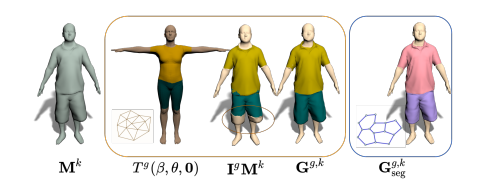
\includegraphics[scale=1]{Images/SizerPic/ParserNet.png}
  \caption{Da sinistra a destra: In input una singola mesh $\left(\mathbf{M}^{k}\right)$, il template dell'abito $\left(T^{g}(\boldsymbol{\beta}, \boldsymbol{\theta}, \mathbf{0})=\right.$ $\left.\mathbf{I}^{g} T(\boldsymbol{\beta}, \boldsymbol{\theta}, \mathbf{0})\right)$, estrazione della mesh del vestito usando $\mathbf{G}^{g, k}=\mathbf{I}^{g} \mathbf{M}^{k}$, mesh multilivello $\left(\mathbf{G}^{g, k}\right)$ registrata a SMPL+G, tutto questo con classi di vestiti munite di specifiche connessioni tra vertici $\mathbf{E}^{g}$, e scansioni segmentate $\mathbf{G}_{\mathrm{seg}}^{g, k}$ con specifiche istanze di connettività tra vertici $\mathbf{E}_{\mathrm{seg}}^{g, k}$.}
  \label{fig:ParserNet}
\end{figure}

\medskip

\subsection{Analisi della body shape svestita}

\medskip

Ai fini di generare una dettagliata body shape svestita, viene prima creata una mesh del corpo lineare, grazie all'utilizzo dei parametri SMPL $\boldsymbol{\theta}$ e $\boldsymbol{\beta}$ ricavati da $f_{w}^{\boldsymbol{\theta}}, f_{w}^{\boldsymbol{\beta}}$. Utilizzando la formulazione di combinazione convessa citata sopra, Body ParserNet trasferisce i vertici della pelle visibile dalla mesh data in input a quella lineare creata, ottenendo così le caratteristiche facciali e relative ai capelli.Successivamente viene scomposta la mesh di input in magliette, pantaloni e forma del corpo svestita utilizzando le 3 sottoreti di ParserNet $\left(f_{w}^{U}, f_{w}^{L}, f_{w}^{B}\right)$ mostrate in figura 1.3.

\medskip

\subsection{Funzione di Loss}

\medskip

La rete ParserNet viene addestrata tramite la funzione di Loss sotto descritta: 
\medskip

\begin{equation*}
\begin{gathered}
\mathcal{L}_{\text {parser }}=w_{3 \mathrm{D}} \mathcal{L}_{3 \mathrm{D}}+w_{\text {norm }} \mathcal{L}_{\text {norm }}+w_{\text {lap }} \mathcal{L}_{\text {lap }}+w_{\text {interp }} \mathcal{L}_{\text {interp }}+w_{\mathrm{w}} \mathcal{L}_{\mathrm{w}} \\
\mathcal{L}_{\text {sizer }}=w_{3 \mathrm{D}} \mathcal{L}_{3 \mathrm{D}}+w_{\text {norm }} \mathcal{L}_{\text {norm }}+w_{\text {lap }} \mathcal{L}_{\text {lap }}+w_{\text {interp }} \mathcal{L}_{\text {interp }}
\end{gathered}
\end{equation*}

\medskip

dove $w_{3 \mathrm{D}}, w_{\text {norm }}, w_{\text {lap }}, w_{\text {interp }}$ and $w_{\mathrm{w}}$ sono i pesi relativi ai vertici di Loss, normali, Laplaciani, di interpenetrazione e di termini di regolarizzazione dei pesi.

\subsubsection{3D Vertex Loss per vestiti}

\medskip

Viene definito $\mathcal{L}_{3 D}$ come una Loss nello spazio $L_{1}$ tra vertici predetti ed effettivi.

\medskip

$$
\mathcal{L}_{3 \mathrm{D}}=\left\|\mathbf{G}_{\mathrm{P}}-\mathbf{G}_{\mathrm{GT}}\right\|_{1} .
$$

\medskip

\subsubsection{3D Vertex Loss corpi svestiti}

Per addestrare $f_{w}^{B}$ (ParserNet specifica per il corpo), viene utilizzata la mesh di input relativa alla pelle come supervisione per prevedere i dettagli personali del soggetto. Si definisce un termine di loss pesato (tramite la distanza geodetica) specifico per ogni classe di vestiti. 

\medskip

$$
\mathcal{L}_{3 \mathrm{D}}^{\text {body }}=\left\|\boldsymbol{w}_{\text {geo }}^{T} \cdot \operatorname{abs}_{i j}\left(\mathbf{G}_{\mathrm{P}}^{s}-\mathbf{I}^{s} \mathbf{M}\right)\right\|_{1}
$$

\medskip

dove $\mathbf{I}^{s}$ è la matrice di indicatori per la specifica regione di pelle e $\boldsymbol{w}_{\text {geo }}$ è un vettore contenente il sigmoide del termine di loss specifico ottenuto tramite distanza geodetica dai vertici appartenenti alla regione relativa alla pelle e non. Il termine di Loss è elevato quando la predizione è molto diversa dalla mesh originale di input $\mathbf{M}$ relativa alle porzioni di pelle visibili, e bassa per quanto riguarda le regioni relative agli indumenti, con una transizione lineare regolata dal termine geodetico. Nella formulazione citata sopra, il termine $\operatorname{abs}_{i j}(\cdot)$ rappresenta un operatore di valore assoluto.  
\medskip

\subsubsection{Normal Loss}

\medskip

Viene definito $\mathcal{L}_{\text {norm }}$ come la differenza in angolo tra la faccia normalizzata reale $\left(\mathbf{N}_{G T}^{i}\right)$ e quella predetta $\left(\mathbf{N}_{P}^{i}\right)$.

\medskip

\subsubsection{Termine di smoothness Laplaciano}

\medskip

Si definisce $\mathbf{L}^{g} \in$ $\mathbb{R}^{m_{g} \times m_{g}}$ come grafo Laplaciano relativo alla mesh dell'abito $\mathbf{G}_{\mathrm{GT}}$, e $\boldsymbol{\Delta}_{\text {init }}=$ $\mathbf{L}^{g} \mathbf{G}_{\mathrm{GT}} \in \mathbb{R}^{m_{g} \times 3}$ come le coordinate differenziali di $\mathbf{G}_{\mathrm{GT}}$, successivamente di computa il termine di smoothness Laplaciano per una predetta mesh $\mathbf{G}_{\mathrm{P}}$ come 

\medskip

$$
\mathcal{L}_{\text {lap }}=\left\|\boldsymbol{\Delta}_{\text {init }}-\mathbf{L}^{g} \mathbf{G}_{\mathrm{P}}\right\|_{2} .
$$

\medskip

\subsubsection{Interpenetration loss}

\medskip

Siccome minimizzare la perdita specifica dei vertici non garantisce che l'indumento predetto sia esterno alla superficie del corpo, viene utilizzato il termine di Interpenetration loss: 

$$
\mathcal{L}_{\text {interp }}=\sum_{(i, j) \in \mathcal{C}\left(\mathbf{B}, \mathbf{G}_{\mathrm{P}}\right)} \mathbb{1}_{d\left(\mathbf{G}_{\mathrm{P}, j}, \boldsymbol{G}_{\mathrm{GT}, j}\right)<d_{\text {tol }}} \operatorname{ReLU}\left(-\mathbf{N}_{i}\left(\mathbf{G}_{\mathrm{P}, j}-\mathbf{B}_{i}\right)\right) / m_{g},
$$

\medskip

Per ogni vertice $\mathbf{G}_{\mathbf{P}, j}$ viene trovato quello più vicino all'interno della body shape svestita predetta  $\mathbf{B}_{i}$ e viene definita una corrispondenza corpo-vestito $\mathcal{C}\left(\mathbf{B}, \mathbf{G}_{\mathrm{P}}\right)$. Se il vertice relativo all'indumento $\mathbf{G}_{\mathrm{P}, j}$ si trova all'interno della superficie del corpo, il modello viene penalizzato mediante la formula sopra descritta.

da notare che $\mathbb{1}_{d\left(\mathbf{G}_{\mathrm{P}, j}, \boldsymbol{G}_{\mathrm{GT}, j}\right)<d_{t o l}}$ attiva il termine di loss solo quando la distanza tra i vertici della mesh del vestito predetta ed i vertici della mesh reale è piccola, ad esempio: $<d_{\text {tol }}$.





\medskip

\subsubsection{Regolarizzazione dei pesi}

\medskip

Per mantenere i dettagli più particolari e fini mentre viene divisa la mesh in input si vuole che i pesi della rete siano sparsi e racchiusi all'interno di un unico cluster. Conseguentemente viene aggiunto un regolarizzatore che penalizza valori elevati per $\mathbf{W}_{i j}$ se la distanza tra $\mathbf{M}_{j}$ ed il vertice $\mathbf{M}_{k}$ (con peso maggiore $k=\arg \max _{j} \mathbf{W}_{i j}$) è grande. Viene definito $d(\cdot, \cdot)$ come distanza Euclidea tra i vertici, allora il regolarizzatore equivale a:

\medskip

$$
\mathcal{L}_{w}=\sum_{i=1}^{m_{g}} \sum_{j \in \mathcal{N}_{i}} \mathbf{W}_{i j} d\left(\mathbf{M}_{k}, \mathbf{M}_{j}\right), k=\arg \max _{j} \mathbf{W}_{i j}
$$

\subsection{Cenno sulle reti neurali utilizzate}

\medskip

Vengono implementate $f_{w}^{\boldsymbol{\theta}}$ e $f_{w}^{\boldsymbol{\beta}}$: reti con con due livelli completamente connessi ed un livello di output lineare. Successivamente si implementa ParserNet $f_{w}^{U}, f_{w}^{L}, f_{w}^{B}$ con 3 livelli completamente connessi. Nello specifico caso di SIZER sono stati utilizzati per gli esperimenti cluster $\left(\mathcal{N}_{i}\right)$ di dimensione 50. 
Inizialmente viene addestrata la rete con classi di vestiti che condividono lo stesso template e successivamente si adattano separatamente per ogni classe $g$.
Per velocizzare il processo di addestramento di ParserNet, si addestra la rete a prevedere $\mathbf{W}^{g}=\mathbf{I}^{g}$, dove $\mathbf{I}^{g}$ riguarda la matrice di indicatori per la classe di vestito $g$.
Grazie a ciò, si inizializza il processo per il quale la rete suddivide il vestito tagliando parte della mesh di input basata sulla matrice di indicatori per ogni vestito.

\medskip

Per la rete di predizione di posa e form, ParserNet usa una dimensione di batch = 8 e una curva di apprendimento di $0.0001$.






\newpage

\section{Codice}

\medskip

Per utilizzare il codice (\url{https://github.com/garvita-tiwari/sizer}) sono necessari come prerequisiti le librerie mesh e kaolin.
In caso di dubbi sui passaggi da seguire, di seguito vengono riportate le istruzioni in maniera semplificata.

\medskip

Di seguito viene illustrata una guida alle installazioni a seconda del sistema operativo di cui si è in possesso.

\medskip

\section{Linux}

\medskip

I comandi mostrati successivamente sono stati testati su una distribuzione Ubuntu 20.04, con la versione di Python 3.6.8.

\medskip

Per prima cosa, bisogna installare le librerie di Boost (\url{https://www.boost.org/users/history/version_1_77_0.html}), in quanto serviranno per l’utilizzo di Psbody-mesh.

\medskip

\begin{itemize}
\item \textit{\$ sudo apt-get install libboost-dev
\item \$ sudo apt install python3.8-venv
\item \$ (opzionale) $>$ mkdir python-venvs
\item \$ (opzionale) $>$ cd python-venvs
\item \$ python3 -m venv --copies <venv\_name>
\item \$ source <venv\_name>/bin/activate
\item \$ mkdir workspace
\item \$ cd workspace/}
\end{itemize}







\medskip

La directory workspace è stata creata per far sì che tutte le librerie che si andranno ad installare si trovino in un unico ambiente di lavoro; durante la loro installazione, quindi, è importante trovarsi nella cartella principale del workspace.


\medskip

\subsubsection{Psbody-mesh}

Questo pacchetto contiene le principali funzioni di manipolazione e visualizzazione di mesh. Richiede Python3.5$+$ e le librerie di Boost.

\medskip





\begin{itemize}
\item \textit{\$ sudo apt install git
\item \$ git clone https://github.com/MPI-IS/mesh
\item \$ cd mesh}
\end{itemize}


\medskip
A questo punto, nel caso in cui la variabile BOOST\_INCLUDE\_DIRS non sia settata, 
bisogna eseguire il seguente comando: 

\code{\$ BOOST\_INCLUDE\_DIRS=/path/to/boost/include make all}




\medskip

Ciò può essere verificato mediante 

\medskip



\code{\$ echo BOOST\_INCLUDE\_IRS.}



\medskip\medskip\medskip

Per ottenere il percorso in cui si trova boost:




\code{\$ whereis boost}



\medskip

Se la compilazione dà errore su Python.h, può significare che dall’installazione di Python manchino i file sorgenti, quindi è necessario cercare il nome della libreria installata e completare l’installazione.

\medskip

\begin{itemize}
\item \textit{\$ sudo apt search libpython
\item \$ sudo apt install libpython3.8-dev}
\end{itemize}




Dopodiché ripetere

\medskip



\code{\$ BOOST\_INCLUDE\_DIRS=/path/to/boost/include make all}



\medskip

A questo punto, l’installazione del pacchetto psbody-mesh è completata e la si può testare mediante \$ make tests.

\medskip

Per ottenere la documentazione e visualizzarla:

\begin{itemize}
\item \textit{\$ make documentation
\item \$ firefox /path/to/mesh/doc/build/html/index.html}
\end{itemize}




\medskip

\subsubsection{Kaolin}

La libreria di NVIDIA Kaolin fa parte di una suite di strumenti per la ricerca sul deep learning 3D. Fornisce una API di PyTorch utile per lavorare con una varietà di rappresentazioni 3D, comprende una raccolta sempre crescente di operazioni ottimizzate per la GPU come rendering differenziabile modulare, conversioni veloci tra rappresentazioni, caricamento dei dati, checkpoint 3D e altro.


\medskip

Requisiti:

\begin{itemize}
\item \textit{Python $>$= 3.6
\item CUDA $>$= 10.0 (con ‘nvcc’ installato)
\item torch $>$= 1.5, $<$= 1.7.1
\item cython == 0.29.20
\item scipy $>$= 1.2.0
\item Pillow $>$= 8.0.0
\item usd-core $>$= 20.11 (opzionale, richiesto per le librerie di Python USD (Universal Scene Description).}

\end{itemize}

\newpage


\subsubsection{CUDA}

\medskip



\code{\$ sudo apt install nvidia-cuda-toolkit}



\medskip

\begin{figure}[ht!]
  \centering
  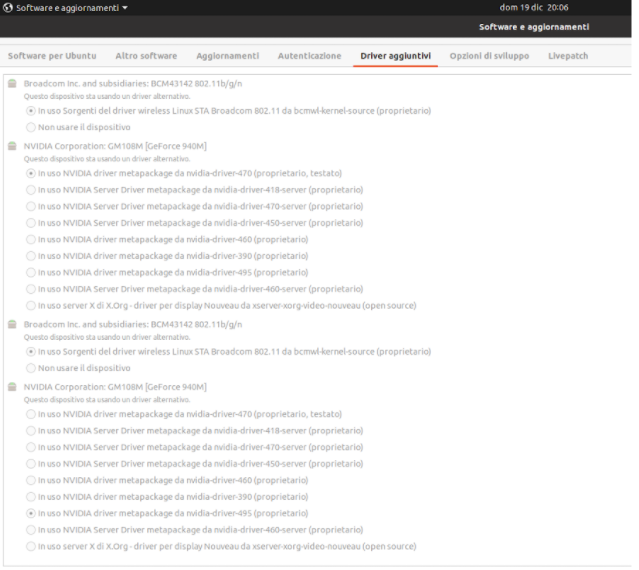
\includegraphics[scale=0.8]{Images/SizerPic/Sizer9.png}
    \label{fig:Sizer9}
\end{figure}

\medskip



\code{\$ sudo apt install cuda}



\medskip

Per assicurarsi di utilizzare la scheda grafica NVIDIA:

\medskip

\code{\$ sudo prime-select intel}

\code{\$ sudo prime-select nvidia}


\medskip

Per avere informazioni sulla scheda grafica:

\medskip



\code{\$ nvidia-smi}



\subsubsection{Installazione di Kaolin}

\medskip

\begin{itemize}
\item \textit{\$ git clone --recursive 
\item \$ cd kaolin
\item \$ git checkout v0.9.0
\item \$ python setup.py develop}
\end{itemize}




website: \url{https://github.com/NVIDIAGameWorks/kaolin}

\medskip

Se durante la fase di setup non dovessero essere trovati torch e/o cython, installarli utilizzando i seguenti comandi:

\medskip

\begin{itemize}
\item \$ pip install torch torchvision
\item \$ pip install Cython
\end{itemize}



\medskip



\code{nvcc warning :} The 'compute\_35', 'compute\_37', 'compute\_50', 'sm\_35', 
'sm\_37' and 'sm\_50' architectures are deprecated, 
and may be removed in a future release (Use -Wno-deprecated-gpu-targets to suppress warning).



\medskip

Questo significa che, per la versione di kaolin 0.9, la GPU risulta deprecata.

\medskip

L’installazione di kaolin v0.1, invece, dà errore perché manca la libreria pptk, la cui wheel non è più reperibile e anche la compilazione dai file sorgenti causa problemi.

\medskip

Kaolin vuole gcc e g$++$ 8 e vuole che la versione di CUDA sia uguale a quella usata da Pytorch, che nell’ultima versione corrisponde a CUDA 10.2.
CUDA 10.2 richiede  gcc e g$++$ 9.

\medskip

Bisogna trovare una versione di PyTorch che usi CUDA 9 (PyTorch 1.2 dovrebbe essere compatibile con CUDA 9), potrebbero tuttavia esserci delle interferenze di compatibilità con gcc v8.

\medskip

Per verificare la possibilità di importare kaolin, si può testare la sua installazione nel seguente modo:

\medskip



\code{\$ python -c "import kaolin; print(kaolin.\_\_version\_\_)"}



\newpage

\subsection{Sizer}

\medskip\medskip\medskip



\code{\$ git clone --recursive https://github.com/garvita-tiwari/sizer}




\medskip\medskip\medskip

Poiché il dataset SIZER include registrazioni sul modello SMPL, bisogna scaricare il modello SMPL \url{https://smpl.is.tue.mpg.de/} e salvarlo nella cartella di sizer training\_{}data.

\medskip\medskip\medskip

\begin{figure}[ht!]
  \centering
  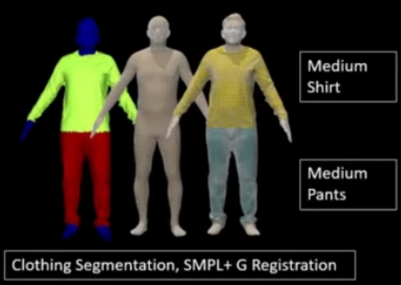
\includegraphics[scale=1]{Images/SizerPic/Sizer2.png}
    \label{fig:Sizer2}
\end{figure}

\medskip\medskip\medskip

Settare

\medskip\medskip\medskip

\code{DATA\_DIR='<downloaded dataset path>/training\_data' in utils/global\_var.py}



\medskip

A questo punto è possibile fare la validazione di ParserNet:




\code{\$ python trainer/parsernet\_eval.py --log\_dir <log\_dir\_path> \-}



\medskip

Si consiglia di salvare i file di log in una cartella dedicata all’interno di quella del progetto Sizer, invece che in trainer, in modo da non contaminare la cartella contenente i file di addestramento.
Se i moduli tensorboardX e ipdb non dovessero essere trovati, procedere alla loro installazione mediante i seguenti comandi:

\medskip

\begin{itemize}
\item \textit{\$ pip install tensorboardX
\item \$ pip install ipdb}
\end{itemize}




\medskip

In caso di errori sugli import, come ad esempio ImportError: cannot import name 'TriangleMesh' from 'kaolin.rep', si consiglia di effettuare il downgrade di torch alla versione 1.4, con la quale il codice sizer è stato testato, oppure, se il problema persiste, passare alla versione 0.1 di kaolin se non è già stato fatto, in quanto dalla versione 0.9 di Kaolin TriangleMesh non esiste più.

\medskip

\begin{itemize}
\item \textit{/kaolin\$ git checkout v0.1
\item /kaolin\$ python setup.py develop}
\end{itemize}



\begin{enumerate}
\item \url{https://githubmemory.com/repo/NVIDIAGameWorks/kaolin/issues/414} 
\item \url{https://github.com/pytorch/pytorch/issues/38090}
\item \url{https://github.com/garvita-tiwari/sizer}
\end{enumerate}




\newpage

\section{Windows}

\medskip

Create a dedicated Python virtual environment and activate it:

\medskip

\code{$>$ conda create -n my\_env (garments)}

\medskip

\code{$>$ conda activate my\_env}



\medskip

Per prima cosa bisogna installare le librerie di Boost.
Si può decidere di seguire le linee guida nel file README \url{https://www.boost.org/users/history/version_1_77_0.html} oppure installarlo da github \url{https://gist.github.com/sim642/29caef3cc8afaa273ce6}

\medskip

Unzip il file boost e seguire le istruzioni presenti in index.html.

\medskip

\subsection{Boost}

\medskip


Leggere il file "Install" per maggiori informazioni.

\medskip

\begin{itemize}
\item Andare nella directory tools -build-.
\item Eseguire bootstrap.bat (sul prompt dei comandi scrivere:  \\ \code{start bootstrap.bat}
\item Eseguire b2install \textit{--prefix=PREFIX} dove PREFIX è la directory dove si vuole installare Boost.Build\\ \code{start b2 install --prefix=.-build}
\end{itemize}


\medskip

Cerca il toolset adatto al compilatore che vuoi utilizzare su Pycharm dalla tabella nel seguente link: (una lista aggiornata è disponibile anche nella documentazione di \textit{Boost.Build})

\medskip

\url{https://www.boost.org/doc/libs/1_77_0/tools/build/doc/html/index.html#bbv2.reference.tools}

\medskip

\subsection{Librerie Boost per GCC}

\medskip

Guida per installare le librerie di Boost per GCC (MinGW): \\
\url{https://gist.github.com/sim642/29caef3cc8afaa273ce6}

\medskip

\subsection{Psbody-mesh}

\medskip

A questo punto, bisogna compilare ed installare il pacchetto Psbody-mesh usando il Makefile:

\medskip

\begin{itemize}
\item cd .path/to/mesh-master
\item make all
\end{itemize}

\medskip

In caso di errori quali

\code{pip uninstall spyder} 

\medskip

\code{pip 10 no longer uninstalls distutils packages}

\medskip 

fare il downgrade a pip 8.1.1.:

\medskip

\code{sudo -H pip3 install pip==8.1.1}




\medskip

Psbody-mesh contiene le principali funzioni di manipolazione e visualizzazione di mesh. Richiede Python3.5$+$ e le librerie di Boost installate seguendo il paragrafo precedente.

\newpage

\subsection{Kaolin}

\medskip

E’ necessaria l’installazione della libreria Kaolin, che può essere effettuata seguendo le linee guida del sito ufficiale: 

\medskip

\url{https://kaolin.readthedocs.io/en/latest/notes/installation.html}

\medskip

La libreria di NVIDIA Kaolin fa parte di una suite di strumenti per la ricerca sul deep learning 3D. Fornisce una API di PyTorch utile per lavorare con una varietà di rappresentazioni 3D, comprende una raccolta sempre crescente di operazioni ottimizzate per la GPU come rendering differenziabile modulare, conversioni veloci tra rappresentazioni, caricamento dei dati, checkpoint 3D e altro.

\medskip

Requisiti:

\begin{itemize}
\item \textit{Python $>$= 3.6
\item CUDA $>$= 10.0 (con nvcc installato)
\item torch $>$= 1.5, $<$= 1.7.1
\item cython == 0.29.20
\item scipy $>$= 1.2.0
\item Pillow $>$= 8.0.0
\item usd-core $>$= 20.11 (opzionale, richiesto per le librerie di Python USD) (Universal Scene Description).}
\end{itemize}







\medskip

E’ possibile eseguire il file di setup di kaolin tramite il terminale di pycharm, all’interno del progetto:
python setup.py install

\medskip



\subsection{Sizer}

\medskip

Scaricare il dataset dalla sezione Data della pagina web di SIZER (\url{http://virtualhumans.mpi-inf.mpg.de/sizer/}), recuperarne il percorso e seguire le istruzioni del README di github (\url{https://github.com/garvita-tiwari/sizer}).



\medskip

\subsection{Installazione dei pacchetti}

\medskip

Per prima cosa è necessario assicurarsi che il pacchetto pip per python 3 sia installato correttamente.

\medskip

In caso contrario, sarà sufficiente eseguire la seguente linea di codice sul terminare direttamente offertoci da pycharm



\code{py -m ensurepip --default-pip}



I pacchetti richiesti dal modello sono 131, facilmente reperibili dal file requirements.txt presente all'interno del github di SIZER. 

\medskip

\url{https://github.com/garvita-tiwari/sizer/blob/master/requirements.txt}

\medskip

Per scaricare le librerie richieste dal file .txt è sufficiente spostarsi, tramite l'utilizzo della shell di python, nella cartella contenente il file requirements.txt ed eseguire il seguente comando:

\medskip

\code{pip install -r requirements.txt}

\medskip

Tuttavia il nome "completo" dei pacchetti inseriti nel documento di testo requirements.txt non corrisponde sempre alla versione richiesta da SIZER.
Per ovviare a questo problema è necessario installare manualmente ogni singolo pacchetto.


\medskip

La maggior parte dei pacchetti è facilmente installabile su pycharm eseguendo il comando pip install [nome pacchetto]

\medskip

Tra questi pacchetti, alcuni necessitano il supporto del terminale di anaconda per essere installati.
Di seguito vengono specificati più comandi d'istallazione per ogni singolo pacchetto in quanto diverse versioni di sistema operativo richiedono diversi comandi compatibili con i rispettivi registri.

\newpage

\begin{tabular}{ |p{8cm}||p{8cm}|  }



\hline
\multicolumn{2}{|c|}{Package List (Windows or Linux)} \\
\hline

\textbf{Nome e versione del pacchetto}& \textbf{Comandi per anaconda}\\
\hline

libwebp==1.2.0=h89dd481\_0&conda install libwebp==1.2.0  \\

\hline

sqlite==3.36.0=hc218d9a\_0&conda install sqlite==3.36.0\\

\hline

  sqlite==3.36.0=hc218d9a\_0&	conda install sqlite==3.36.0\\
\hline

libwebp-base==1.2.0=h27cfd23\_0&conda install libwebp-base==1.2.0\\
\hline

  xz==5.2.5=h7b6447c\_0&	conda install xz==5.2.5\\
\hline

  yaml==0.2.5=h516909a\_0&	conda install yaml==0.2.5\\
\hline

  pexpect==4.8.0=pypi\_0&	conda install pexpect==4.8.0\\
\hline


  jpeg==9d=h7f8727e\_0&	conda install jpeg==9d\\
\hline


  numpy==1.21.2=py38h20f2e39\_0&	conda install numpy==1.21.2\\
\hline



  giflib==5.2.1=h7b6447c\_0&conda install giflib==5.2.1\\
\hline


  libuv==1.40.0=h7b6447c\_0&	conda install libuv==1.40.0\\
\hline



  libtiff==4.2.0=h85742a9\_0&	conda install libtiff==4.2.0\\
\hline


  mkl\_fft==1.3.1=py38hd3c417c\_0&	conda install mkl\_fft==1.3.1\\
\hline


  lcms2==2.12=h3be6417\_0&	conda install lcms2==2.12\\
\hline


  mkl\_random==1.2.2=py38h51133e4\_0&	conda install mkl\_random==1.2.2\\
\hline


  mkl-service==2.4.0=py38h7f8727e\_0&	conda install mkl-service==2.4.0\\
\hline


  cudatoolkit==10.2.89=hfd86e86\_1&	conda install cudatoolkit==10.2.89\\
\hline


  scikit-image==0.18.3=pypi\_0&	conda install scikit-image==0.18.3\\
\hline


  tk==8.6.11=h1ccaba5\_0&	conda install tk==8.6.11\\
\hline


  numpy-base==1.21.2=py38h79a1101\_0&	conda install numpy-base==1.21.2\\
\hline


  lz4-c==1.9.3=h295c915\_1&	conda install lz4-c==1.9.3\\
\hline



   zstd==1.4.9=haebb681\_0&	conda install zstd==1.4.9\\
\hline


   libpng==1.6.37=hbc83047\_0&	conda install libpng==1.6.37\\
\hline


   openssl==1.1.1l=h7f8727e\_0&	conda install openssl==1.1.1l\\
\hline


 torchvision==0.8.2=cpu\_py38ha229d99\_0&	conda install -c pytorch-lts torchvision\\
\hline



  cachetools==4.2.4=pypi\_0&	conda install -c quantopian cachetools\\
\hline


  pytorch==1.7.1=py3.8\_cuda10.2.89\_cudnn7.6.5\_0&	conda install -c fastchan pytorch\\
\hline

libffi==3.3=he6710b0\_2&conda install -c conda-forge libffi \hline conda install -c conda-forge/label/gcc7 libffi \hline conda install -c conda-forge/label/broken libffi \hline conda install -c conda-forge/label/cf201901 libffi \hline conda install -c conda-forge/label/cf202003 libffi\\

\hline

  liblapack==3.9.0=12\_linux64\_mkl&	conda install -c conda-forge liblapack \hline 	conda install -c conda-forge/label/broken liblapack \hline	conda install -c conda-forge/label/cf202003 liblapack\\
\hline

  freetype==2.11.0=h70c0345\_0&	conda install -c conda-forge freetype \hline 	conda install -c conda-forge/label/gcc7 freetype \hline	conda install -c conda-forge/label/cf201901 freetype \hline	conda install -c conda-forge/label/cf202003 freetype\\
\hline

  Shapely-1.8.0&	conda install -c conda-forge shapely \hline	conda install -c conda-forge/label/gcc7 shapely \hline	conda install -c conda-forge/label/cf201901 shapely \hline	conda install -c conda-forge/label/cf202003 shapely \hline	conda install -c conda-forge/label/shapely\_dev shapely\\
\hline



  igl==2.2.1=py38h52fb889\_1&	conda install -c conda-forge igl \hline 	conda install -c conda-forge/label/cf202003 igl\\
\hline

  ca-certificates==2021.10.8=ha878542\_0&	conda install -c conda-forge ca-certificates \hline 	conda install -c conda-forge/label/gcc7 ca-certificates \hline 	conda install -c conda-forge/label/broken ca-certificates \hline 	conda install -c conda-forge/label/cf201901 ca-certificates \hline	conda install -c conda-forge/label/cf202003 ca-certificates\\
\hline


\end{tabular}


\newpage

Per quanto riguarda i seguenti pacchetti è necessariamente richiesto Linux come sistema operativo.

\medskip

\begin{tabular}{ |p{8cm}||p{8cm}|  }



\hline
\multicolumn{2}{|c|}{Package List (Linux only)} \\
\hline

Nome e versione del pacchetto& comandi per anaconda\\
\hline

  libgomp==9.3.0=h5101ec6\_17   &	conda install -c conda-forge libgomp\hline
	conda install -c conda-forge/label/broken libgomp \hline
	conda install -c conda-forge/label/cf202003 libgomp\\
\hline


  libstdcxx-ng==9.3.0=hd4cf53a\_17  &	conda install -c conda-forge libstdcxx-ng\hline conda install -c conda-forge/label/gcc7 libstdcxx-ng \hline conda install -c conda-forge/label/broken libstdcxx-ng \hline conda install -c conda-forge/label/cf201901 libstdcxx-ng \hline	conda install -c conda-forge/label/cf202003 libstdcxx-ng\\
\hline


  ld\_impl\_linux-64==2.35.1=h7274673\_9  &	conda install -c conda-forge ld\_impl\_linux-64\hline conda install -c conda-forge/label/broken ld\_impl\_linux-64\hline conda install -c conda-forge/label/cf202003 ld\_impl\_linux-64\\
\hline


  \_openmp\_mutex==4.5=1\_gnu  &	conda install -c conda-forge \_openmp\_mutex\hline

	conda install -c conda-forge/label/cf202003 \_openmp\_mutex\\
\hline

		
  libgfortran5==11.2.0=h5c6108e\_11 &
	conda install -c conda-forge libgfortran5\hline

	conda install -c conda-forge/label/broken libgfortran5\\
\hline


  libcblas==3.9.0=12\_linux64\_mkl &
	conda install -c nogil libcblas\hline

	conda install -c cctbx202112 libcblas\\
\hline


  libgfortran-ng==11.2.0=h69a702a\_11  &
	conda install -c conda-forge libgfortran-ng\hline

	conda install -c conda-forge/label/broken libgfortran-ng\hline

	conda install -c conda-forge/label/cf201901 libgfortran-ng\hline

	conda install -c conda-forge/label/cf202003 libgfortran-ng\\
\hline


ncurses==6.3=h7f8727e\_2  &
	conda install -c conda-forge ncurses\hline

	conda install -c conda-forge/label/gcc7 ncurses\hline

	conda install -c conda-forge/label/cf201901 ncurses\hline

	conda install -c conda-forge/label/cf202003 ncurses\\
\hline


  readline==8.1=h27cfd23\_0 &
	conda install -c conda-forge readline\hline

	conda install -c conda-forge/label/gcc7 readline\hline

	conda install -c conda-forge/label/cf201901 readline\hline

	conda install -c conda-forge/label/cf202003 readline\\
\hline

  
  nvidiacub==1.10.0=0 &	conda install -c bottler nvidiacub\\
\hline


  libgcc-ng==9.3.0=h5101ec6\_17  &
	conda install -c conda-forge libgcc-ng\hline

	conda install -c conda-forge/label/gcc7 libgcc-ng\hline

	conda install -c conda-forge/label/broken libgcc-ng\hline

	conda install -c conda-forge/label/cf201901 libgcc-ng\hline

	conda install -c conda-forge/label/cf202003 libgcc-ng\\
\hline


  pytorch3d==0.5.0=py38\_cu102\_pyt171  &
	conda install -c pytorch3d pytorch3d\hline

	conda install -c pytorch3d/label/archived pytorch3d\\
\hline


\end{tabular}

\medskip

Alcuni di questi pacchetti sono necessari per abilitare la fase di training su Pycharm.

































































